\section{PRF(UHF)组合:使用 UHF 构建 MAC}

现在,我们想要表明,只要哈希是一个计算性 UHF,我们就能利用先哈希后 PRF 范式产生一个安全的 PRF。ECBC、NMAC 和 $\mathrm{PMAC}_0$ 都可以被看作是这种构造的实例,它们的安全性很容易由先哈希后 PRF 范式的安全性推出。

\begin{figure}
  \centering
  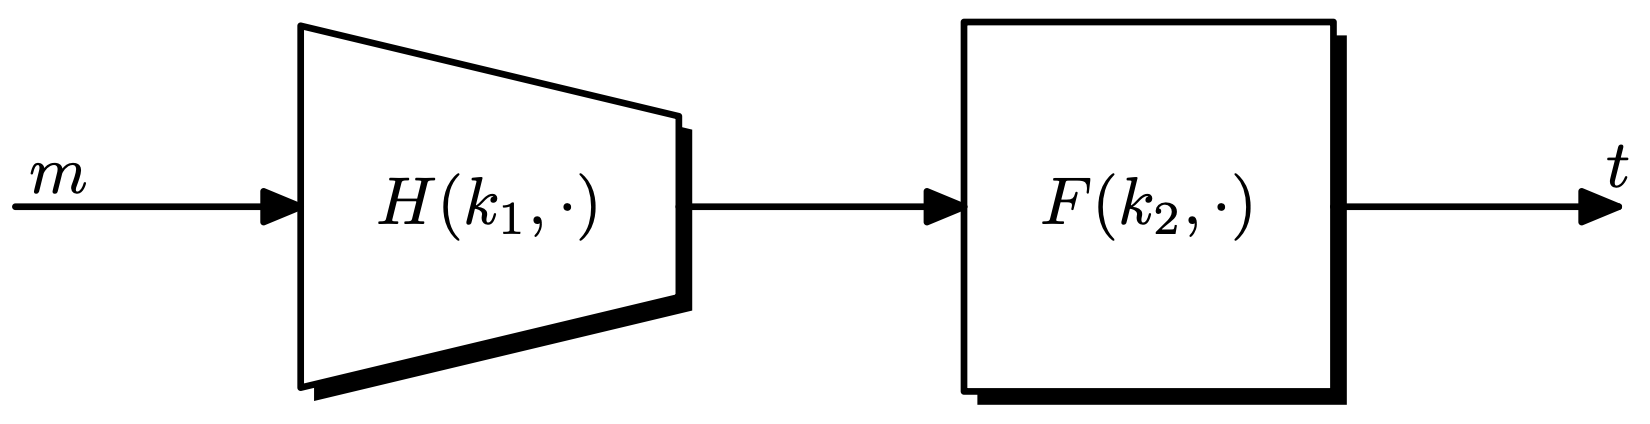
\includegraphics[width=0.5\linewidth]{figures/chapter7/fig3.png}
  \caption{PRF(UHF)组合:MAC签名}
  \label{fig:7-3}
\end{figure}

令 $H$ 是一个定义在 $(\mathcal{K}_H,\mathcal{M},\mathcal{X})$ 上的带密钥哈希函数,令 $F$ 是一个定义在 $(\mathcal{K}_F,\mathcal{X},\mathcal{T})$ 上的 PRF。同之前一样,我们假设 $\mathcal{M}$ 中的消息比 $\mathcal{X}$ 中的元素长得多,因此 $H$ 可以将较长的输入哈希成较短的摘要。我们下面通过将哈希函数 $H$ 与 PRF $F$ 相结合,来构建一个新的 PRF $F'$,如图 \ref{fig:7-3} 所示。更确切地说,$F'$ 的定义如下:
\begin{equation}\label{eq:7-18}
F'\big((k_1,k_2),\,m\big)=F\big(k_2,\,H(k_1,m)\big)
\end{equation}
我们将 $F'$ 称为 \textbf{$F$ 和 $H$ 的组合 (composition of $F$ and $H$)}。它接受 $\mathcal{M}$ 中的输入,使用一个 $\mathcal{K}_H\times\mathcal{K}_F$ 中的密钥 $(k_1,k_2)$,并输出 $\mathcal{T}$ 中的元素。于是,我们就得到了一个输出空间与底层的 $F$ 相同的 PRF,但是他接受更长的输入。下面的定理表明,$F'$ 是一个安全的 PRF。

\begin{theorem}[PRF(UHF)组合]\label{theo:7-7}
假设 $H$ 是一个计算性 UHF,$F$ 是一个安全 PRF,则式 \ref{eq:7-18} 中定义的 $F'$ 是一个安全的 PRF。
\begin{quote}
特别地,对于每个按照攻击游戏 \ref{game:4-2} 攻击 $F'$ 的 PRF 对手 $\mathcal{A}$,假设他最多能够向其挑战者发起 $Q$ 次查询,则必然存在一个攻击 $F$ 的 PRF 对手 $\mathcal{B}_F$ 和一个攻击 $H$ 的 UHF 对手 $\mathcal{B}_H$,其中 $\mathcal{B}_F$ 和 $\mathcal{B}_H$ 都是围绕 $\mathcal{A}$ 的基本包装器,满足:
\end{quote}
\begin{equation}\label{eq:7-19}
{\rm PRF}\mathsf{adv}[\mathcal{A},F']\leq{\rm PRF}\mathsf{adv}[\mathcal{B}_F,F]+{(Q^2/2)}\cdot{\rm UHF}\mathsf{adv}[\mathcal{B}_H,H]
\end{equation}
\begin{quote}
更一般地,必然存在一个 $Q$ 次查询 UHF 对手 $\mathcal{B}_H'$,其中 $\mathcal{B}_H'$ 是一个围绕 $\mathcal{A}$ 的基本包装器,满足:
\end{quote}
\begin{equation}\label{eq:7-20}
{\rm PRF}\mathsf{adv}[\mathcal{A},F']\leq{\rm PRF}\mathsf{adv}[\mathcal{B}_F,F]+{\rm MUHF}\mathsf{adv}[\mathcal{B}_H',H]
\end{equation}
\end{theorem}

为了理解为什么 $H$ 一定要是一个 UHF,我们不妨先假设它不是的情况。特别地,我们假设很容易找到互不相同的 $m_0,m_1\in\mathcal{M}$,即使不知道 $k_1$ 也能使得 $H(k_1,m_0)=H(k_1,m_1)$。这种 $H$ 的碰撞意味着$F'((k_1,k_2),\,m_0)=F'((k_1,k_2),\,m_1)$。但是,$F'$ 显然不是一个安全 PRF,因为对手可以要求 $t_0:=F'((k_1,k_2),\,m_0)$,$t_1:=F'((k_1,k_2),\,m_1)$,然后只在 $t_0=t_1$ 时输出 $1$。当与 $F'$ 交互时,对手总是会输出 $1$,但对于一个随机函数,他更常会输出 $0$。 因此,对手就能够成功地将 $F'$ 和一个随机函数区分开来。上述论证表明,要使 $F'$ 成为一个 PRF,它必须保证在不知道 $k_1$ 的情况下很难找到 $H$ 的碰撞。换句话说,要使 $F'$ 成为一个 PRF,哈希函数 $H$ 必须是一个 UHF。定理 \ref{theo:7-7} 表明,这个条件就足够了。

\begin{remark}\label{remark:7-2}
定理 \ref{theo:7-7} 中的约束是严格的。考虑一下我们在 \ref{subsec:7-2-1} 小节中讨论过的 UHF $H_{\rm poly}$。更具体地说,让我们假设 $\ell=2$,此时 $H_{\rm poly}$ 的消息空间是 $\mathbb{Z}^2_p$,输出空间是 $\mathbb{Z}_p$,碰撞概率是 $\epsilon={1}/{p}$。在练习 7.26 中,我们会要求你证明,对于任意固定的哈希密钥 $k_1$,在 $H_{\rm poly}(k_1,\cdot)$ 的 $\sqrt{p}$ 个随机输入中,碰撞发生的概率有一个常数下界;此外,对于任何这样的碰撞,我们都可以有效地恢复密钥 $k_1$。现在,考虑由使用 $H_{\rm poly}$ 的 PRF(UHF) 组合得到的 MAC。如果对手发现两条消息 $m_0,m_1$ 能够引发内部碰撞(即导致 $H_{\rm poly}$ 的碰撞),它就能够恢复 $H_{\rm poly}$ 的密钥,继而破解 MAC。这表明,式 \ref{eq:7-19} 中出现的 ${(Q^2/2)\epsilon}$ 项没有办法被大幅度的改进。
\end{remark}

\begin{snote}[定理 \ref{theo:7-7} 的证明。]
我们现在证明,对 $F$ 和 $H$ 的组合能够得到一个安全的 PRF。
\end{snote}

\begin{proof}[证明思路]
令 $\mathcal{A}$ 是一个有效 PRF 对手,它就 $F'$ 进行攻击游戏 \ref{game:4-2}。我们下面推导 ${\rm PRF}\mathsf{adv}[\mathcal{A},F']$ 的上界。也就是说,我们想要对 $\mathcal{A}$ 区分 $F'$ 和 ${\rm Funs}[\mathcal{M},\mathcal{X}]$ 中的一个真随机函数的能力进行约束。同之前一样,我们首先注意到,用一个真随机函数 $f$ 替换底层的安全 PRF $F$ 并不会对 $\mathcal{A}$ 的优势造成太大的改变。接下来,我们将表明,由于 $f$ 是一个真随机函数,所以 $\mathcal{A}$ 能将 $F':=f(H(k_1,m))$ 与一个真随机函数区分开来的唯一方法是,他能找到两个输入 $m_0,m_1$ 使得 $H(k_1,m_0)=H(k_1,m_1)$。但由于 $H$ 是一个计算性 UHF,所以 $\mathcal{A}$ 无法有效地找到 $H(k_1,\cdot)$ 的碰撞。因此,将 $F'$ 和一个随机函数区分开来是不可能的。
\end{proof}

\begin{proof}
我们首先证明式 \ref{eq:7-20},那么根据引理 \ref{lemma:7-1},我们可以由式 \ref{eq:7-20} 推出式 \ref{eq:7-19}。我们令 $\mathcal{A}$ 在三个游戏中与三个密切相关的挑战者交互。对于 $j=0,1,2$,我们定义 $W_j$ 为 $\mathcal{A}$ 在游戏 $j$ 结束时输出 $1$ 的事件。

\vspace{5pt}

\noindent\textbf{游戏 $\mathbf{0}$}。
游戏 $0$ 的挑战者与就 $F'$ 进行攻击游戏 \ref{game:4-2} 的实验 $0$ 的挑战者是相同的。不失一般性,我们假设 $\mathcal{A}$ 对 $F'$ 的查询是各不相同的。挑战者的工作方式如下:

\vspace{5pt}

\hspace*{5pt} 选取 $k_1\overset{\rm R}\leftarrow\mathcal{K}_H$,$k_2\overset{\rm R}\leftarrow\mathcal{K}_F$\\
\hspace*{26pt} 当从 $\mathcal{A}$ 处收到第 $i$ 个查询 $m_i\in\mathcal{M}$ ($i=1,2,\dots$) 时:\\
\hspace*{50pt} 令 $x_i\leftarrow H(k_1,\,m_i)$\\
\hspace*{50pt} 令 $t_i\leftarrow F(k_2,\,x_i)$\\
\hspace*{50pt} 将 $t_i$ 发送给对手

\vspace{5pt}

\noindent
注意,由于 $\mathcal{A}$ 的查询被确保是各不相同的,因此所有的 $m_i$ 值也是各不相同的。

\vspace{5pt}

\noindent\textbf{游戏 $\mathbf{1}$}。
与之前一样,现在,我们打出 ``PRF牌",用 ${\rm Funs}[\mathcal{X},\mathcal{T}]$ 中的一个真随机函数 $f$ 代替函数 $F(k_2,\cdot)$,我们把它实现为一个忠实的侏儒(见 \ref{subsec:4-4-2} 小节)。那么,游戏 $1$ 中挑战者的工作方式如下:

\vspace{5pt}

\hspace*{5pt} 选取 $k_1\overset{\rm R}\leftarrow\mathcal{K}_H$,$t_1',\dots,t_Q'\overset{\rm R}\leftarrow\mathcal{T}$\\
\hspace*{26pt} 当从 $\mathcal{A}$ 处收到第 $i$ 个查询 $m_i\in\mathcal{M}$ ($i=1,2,\dots$) 时:\\
\hspace*{50pt} 令 $x_i\leftarrow H(k_1,\,m_i)$\\
\hspace*{50pt} 令 $t_i\leftarrow t_i'$\\
\hspace*{1pt} ($*$)
\hspace*{28pt} 如果存在某个 $j<i$ 使得 $x_i=x_j$,则令 $t_i\leftarrow t_j$\\
\hspace*{50pt} 将 $t_i$ 发送给对手

\vspace{5pt}

\noindent
对于 $i = 1,\dots,Q$,$t_i'$ 会事先被选为 $t_i=f(x_i)$ 的默认随机值。尽管消息是各不相同的,但它们的哈希值可能存在重复。因此,标有 ($*$) 的一行确保挑战者模仿了一个 ${\rm Funs}[\mathcal{X},\mathcal{T}]$ 中函数——如果两个哈希值发生冲突,挑战者就对两个查询给出同样的应答。和往常一样,我们可以很容易地证明,存在一个 PRF 对手 $\mathcal{B}_F$,其运行时间与 $\mathcal{A}$ 差不多,使得:
\begin{equation}\label{eq:7-21}
\big\lvert\Pr[W_1]-\Pr[W_0]\big\rvert={\rm PRF}\mathsf{adv}[\mathcal{B}_F,F]
\end{equation}

\noindent\textbf{游戏 $\mathbf{2}$}。
接下来,我们通过删去标有 ($*$) 的那一行,使我们的侏儒变得健忘。

利用 $\mathcal{A}$ 无法有效地找到 $H$ 的碰撞这一事实,我们说明 $\mathcal{A}$ 无法区分游戏 $1$ 和游戏 $2$。正是地说,我们利用差分引理(定理 \ref{theo:4-7})来分析 $|\Pr[W_2]-\Pr[W_1]|$ 的值。令 $Z$ 为游戏 $2$ 中存在某个 $i\neq j$ 使得 $x_i=x_j$ 的事件。那么,事件 $Z$ 本质上就是就 $H$ 的多次查询 UHF 游戏(攻击游戏 \ref{game:7-2})的获胜条件。特别地,存在一个 $Q$ 次查询 UHF 对手 $\mathcal{B}_H'$,它能以 $\Pr[Z]$ 的概率赢得攻击游戏 \ref{game:7-2}。对手 $\mathcal{B}_H'$ 简单地模仿游戏 $2$ 中的挑战者,直至 $\mathcal{A}$ 停机,然后输出 $\mathcal{A}$ 的查询 $m_1,m_2,\dots$ 作为其最终的列表。这之所以是有效的,是因为在游戏 $2$ 中,挑战者并不需要真正获取到哈希密钥 $k_1$,他只是用 $\mathcal{T}$ 中的一个随机元素来响应每次查询。因此,对手 $\mathcal{B}_H'$ 可以在不知道 $k_1$ 的情况下轻松地模仿游戏 $2$ 中的挑战者。根据 $Z$ 的定义,我们有${\rm MUHF}\mathsf{adv}[\mathcal{B}_H',H]=\Pr[Z]$。

显然,除非事件 $Z$ 发生,否则游戏 $1$ 和游戏 $2$ 的进程是完全相同的;特别是,当且仅当 $W_1\land\bar{Z}$ 发生时,$W_2\land\bar{Z}$ 才会发生。应用差分定理,我们可得:
\begin{equation}\label{eq:7-22}
\big\lvert\Pr[W_2]-\Pr[W_1]\big\rvert\leq\Pr[Z]={\rm MUHF}\mathsf{adv}[\mathcal{B}_H',H]
\end{equation}

\noindent\textbf{完成证明}。
游戏 $2$ 的挑战者为 $\mathcal{A}$ 模拟了 ${\rm Funs}[\mathcal{M},\mathcal{T}]$ 中的一个真随机函数,因此与就 $F'$ 的实验 $1$ 的 PRF 挑战者是相同的。于是,我们得到:
\[
\begin{aligned}
{\rm PRF}\mathsf{adv}[\mathcal{A},F']
&=\big\lvert\Pr[W_2]-\Pr[W_0]\big\rvert\\
&\leq\big\lvert\Pr[W_2]-\Pr[W_1]\big\rvert+\big\lvert\Pr[W_1]-\Pr[W_0]\big\rvert\\
&={\rm PRF}\mathsf{adv}[\mathcal{B}_F,F]+{\rm MUHF}\mathsf{adv}[\mathcal{B}_H',H]
\end{aligned}
\]
这就证明了式 \ref{eq:7-20},正如定理所要求的。
\end{proof}

\subsection{使用 PRF(UHF)组合:ECBC 和 NMAC 的安全性}\label{subsec:7-3-1}

使用定理 \ref{theo:7-7},我们可以快速地证明许多 MAC 构造的安全性,事实上,我们只需证明 MAC 算法可以被分解为一个 PRF 与一个 UHF 的组合。我们首先说明 ECBC 和 NMAC 可以被这样描述,并在接下来的两个小节中给出更多的例子。

ECBC 和 NMAC 的安全性直接来源于 PRF(UHF) 组合。这两种方案的证明过程如下:
\begin{itemize}
	\item 首先,我们证明了 CBC 和级联都是无前缀安全的 PRF(定理 \ref{theo:6-3} 和 定理 \ref{theo:6-4})。我们观察到,这两者都是可扩展的。
	\item 接着,我们表明了,任何可扩展的无前缀安全的 PRF 也都是计算性 UHF(定理 \ref{theo:7-3})。特别是,CBC 和级联都是计算性 UHF。
	\item 最后,我们证明了,一个计算性 UHF 和一个 PRF 的组合是一个安全的 PRF(定理 \ref{theo:7-7})。因此,ECBC 和 NMAC 都是安全的 PRF。
\end{itemize}
更一般地,加密 PRF 构造(定理 \ref{theo:6-5})是 PRF(UHF) 组合的一个实例,因此,对它的证明可以由定理 \ref{theo:7-7} 得到。ECBC 和 NMAC 的安全性定理(定理 \ref{theo:6-6} 和定理 \ref{theo:6-7})中的具体约束可以通过将式 \ref{eq:7-10} 和式 \ref{eq:7-11} 分别接驳到式 \ref{eq:7-20} 中得到。

我们可以通过直接证明 CBC 和级联都是计算性 UHF 来简化 ECBC 和 NMAC 的安全性证明。我们已经证明了它们都是无前缀安全的 PRF,这比上面的我们的需求还要强。然而,这个更强的结果还能帮助我们构建其他的安全 MAC,比如 CMAC(见 \ref{sec:6-7} 节)。

\subsection{将 PRF(UHF)组合与多项式 UHF 一起使用}\label{subsec:7-3-2}

当然,我们可以将 PRF(UHF) 构造与一个基于多项式的 UHF——比如 $H_{\rm poly}$——一起使用。视乎底层硬件,这种构造可能比 ECBC,NMAC 或 $\mathrm{PMAC}_0$ 要快得多,尤其是对于很长的消息。

回顾一下,$H_{\rm poly}$ 将 $\mathbb{Z}^{\leq\ell}_p$ 中的消息哈希为 $\mathbb{Z}_p$ 上的摘要,其中 $p$ 是一个素数。现在,我们很可能想使用一个分组长度为 $n$ 比特的分组密码作为这里的 PRF,比如 AES。

为了使其发挥作用,我们必须以某种方式进行调整,使哈希函数的摘要空间等于 PRF 的输入空间。一种方法是选定一个素数 $p$,使其比 $2^n$ 稍小一点。这样,我们就可以将哈希摘要编码为 PRF 的输入。尽管这种方法是可行的,但是它有一个问题,就是我们必须将哈希函数的输入视为 $\mathbb{Z}_p$ 上元素的序列。因此,比如说,在 AES 中,$n=128$,我们可以选择一个 $128$ 比特的素数。但这样一来,哈希函数的输入就需要被拆分为——比如,$120$ 比特(即$15$字节)——的分组。如果我们也能直接将输入的哈希值处理成 $n$ 比特分组的序列,那就更方便了。练习 7.23 的 (d) 部分将展示如何做到这一点,它会使用一个比 $2^n$ 稍\emph{大}一点的素数。还有一种方法是,我们不把哈希值建立在素数 $p$ 的模算术运算上,而是建立在有限域 $\mathrm{GF}(2^n)$ 的算术运算上,如备注 \ref{remark:7-1} 所述。

\subsection{使用 PRF(UHF)组合:$\mathrm{PMAC}_0$的安全性}\label{subsec:7-3-3}

接下来,我们表明,\ref{sec:6-11} 节中讨论的 $\rm PMAC_0$ 构造也是 PRF(UHF) 组合的一个实例。回顾一下,$\rm PMAC_0$ 由两个 PRF 构建而成,$F_1$ 定义在 $(\mathcal{K}_1,\mathbb{Z}_p,\mathcal{Y})$ 上,$F_2$ 定义在 $(\mathcal{K}_2,\mathcal{Y},\mathcal{Z})$ 上,其中 $\mathcal{Y}:=\{0,1\}^n$。

在此,读者应当回顾一下 $\rm PMAC_0$ 的构造,特别是图 \ref{fig:6-9}。我们可以看到,$\rm PMAC_0$ 在本质上就是 PRF $F_2$ 和某个带密钥哈希函数 $\widehat{H}$ 的组合,后者也就是图 \ref{fig:6-9} 的其余部分。

现在,我们的目标是证明 $\widehat{H}$ 是一个计算性 UHF。为了做到这一点,我们注意到,$\widehat{H}$ 可以被看作是 \ref{subsec:7-2-3} 小节中的异或哈希构造的一个实例,应用于定义在 $(\mathbb{Z}_p\times\mathcal{K}_1,\mathbb{Z}_p\times\{1,\dots,\ell\},\mathcal{Y})$ 上的 PRF $F'$,如下所示:
\[
F'\big((k,k_1),\,(a,i)\big)=F_1(k_1,\,a+i\cdot k)
\]

所以,我们只需证明 $F'$ 是一个安全的 PRF。但事实证明,我们可以将 $F'$ 本身视作 PRF(UHF) 组合的一个实例。也就是说,它是 PRF $F_1$ 与定义在 $(\mathbb{Z}_p,\mathbb{Z}_p\times\{1,\dots,\ell\},\mathbb{Z}_p)$ 上的带密钥哈希函数 $H$ 的组合,其中$H(k,(a,i)):=a+i\cdot k$。然而,$H$ 只是 $H_{\rm fpoly}$ 的一个实例(见 \ref{subsec:7-2-1})。特别是,根据练习 7.16 的结论,$H$ 是一个 ${1}/{p}$-UHF。

根据上述观察,我们就可以确定 $\rm PMAC_0$ 的安全性。定理 \ref{theo:6-11} 中的具体的安全约束(式 \ref{eq:6-28})来自于定理 \ref{theo:7-7} 中的安全边界(式 \ref{eq:7-20})以及练习 7.27 中对异或哈希的更精确的分析。

在 $\rm PMAC_0$ 的设计中,我们假设 $F_1$ 的输入空间等于 $\mathbb{Z}_p$。虽然这简化了分析,但却使它在实践中更难操作。正如 \ref{subsec:7-3-2} 小节所述,我们更倾向于使用输入分组长度为 $n$ 比特的分组密码定义的 PRF,比如 AES。我们可以应用 \ref{subsec:7-3-2} 小节中所讨论的技术来得到 $\rm PMAC_0$ 的一个变体,其输入空间由 $n$ 比特分组的序列,而不是 $\mathbb{Z}_p$ 中元素的序列组成。一个例子可见练习 7.25。